\documentclass[12pt]{article}

\usepackage{graphicx}
\usepackage[margin=1.0in]{geometry}
\usepackage{amsmath}
\usepackage{cases}
\usepackage{amsfonts}
\usepackage{amssymb}
\usepackage{grffile}
\usepackage{setspace}
\usepackage{listings}

\setlength\parindent{0pt}

\author{Xiaohui Chen \\EID: xc2388}
\title{PHY 362K Homework 3}

\begin{document}
\maketitle
\begin{spacing}{2.0}

\section{} %1

\subsection*{(a)}
From equation 1.25 in lecture note and the reduced mass correction, we get that $E_n=-\frac{1}{2} \left( \frac{m_e}{\hbar^2} \right) \left(\frac{e^2}{4\pi\epsilon_0} \right)^2 \left(\frac{m_p}{m_p+m_e}\right) \frac{Z^2}{n^2}$

We know that $m_p=1.672621*10^{-27} kg$ and $m_e=9.109*10^{-31} kg$

$\therefore \frac{m_p}{m_p+m_e}=0.999456$

We also know that $Z=2$

Plug in all the values of the constants, we get

$\boxed{E_1=-54.393147 eV}$

$\boxed{E_2=-13.598287 eV}$

$\boxed{E_3=-6.043683 eV}$

Equation 1.9 tells us $\frac{1}{\lambda_{nn'}}=\frac{E_n-E_{n'}}{hc}$, where $hc=1240 eV\cdot nm=1.24*10^{-4} eV \cdot cm$

Therefore, in unit of $cm^{-1}$, we redefine energy $E'_n=\frac{E_n-E_{1}}{hc}$

$\therefore \boxed{E'_1=0 cm^{-1}}$

$\boxed{E'_2=328991 cm^{-1}}$

$\boxed{E'_3=389915 cm^{-1}}$

\subsection*{(b)}
The calculated energies and measured energies are shown in the table below:

\begin{tabular}{|c|c|c|c|}
  \hline
  % after \\: \hline or \cline{col1-col2} \cline{col3-col4} ...
  n & $E'_{n-calculated}$ ($cm^{-1}$) & $E'_{n-measured}$ ($cm^{-1}$) & fractional difference=$\frac{|E'_{n-measured}- E'_{n-calculated}|}{E'_{n-measured}}$ \\
  \hline
  1 & 0 & 0 & N/A \\
  \hline
  2 & 328991 & 329179.76197 & 0.000574019 \\
  \hline
  3 & 389915 & 390140.964175 & 0.000579109 \\
  \hline
\end{tabular}

The fractional difference is also shown on the table above

\subsection*{(c)}
The Balmer-$\alpha$ transition is the transition between $n=3$ and $n=2$

$\frac{1}{\lambda_{32}}= E'_{3-measured}-E'_{2-measured}= 60961.2 cm^{-1}$

$\therefore \lambda_{32} \approx 164.039 nm$

According to the electromagnetic spectrum, the light emitted is within the ultraviolet region. Therefore the light is not visible

\section{} %2

\subsection*{(a)}
This part is omitted because we don't have to turn in any work for this part

\subsection*{(b)}
The Schrodinger equation for hydrogen eigenvalue problem is:

$\left[ -\frac{\hbar^2}{2m_e} \frac{d^2}{dr^2} + V_{eff}(r) \right] u(r)=Eu(r)$ where $V_{eff}=-\frac{e^2}{4\pi \epsilon_0 r}+\frac{l(l+1)\hbar^2}{2m_er^2}$

When $\rho=\frac{r}{a_0}$ and $\epsilon=\frac{E}{e^2/4\pi \epsilon_0 a_0}$, we get

$\rho^2=\frac{r^2}{a_0^2}$, then $dr^2=a_0^2 d\rho^2$

We also know that $a_0=\frac{4\pi \epsilon_0 \hbar^2}{me^2}$, which means $\frac{e^2}{4\pi \epsilon_0 a_0}= \frac{\hbar^2}{m_e a_0^2}$

$\therefore \left[ -\frac{\hbar^2}{2m_e a_0^2} \frac{d^2}{d\rho^2} -\frac{e^2}{4\pi \epsilon_0 a_0\rho}+\frac{l(l+1)\hbar^2}{2m_e a_0^2\rho^2} \right] u(\rho)=Eu(r)$

$\left[ -\frac{1}{2} \frac{d^2}{d\rho^2} -\frac{1}{\rho}+\frac{l(l+1)}{2\rho^2} \right] u(\rho)=\frac{E}{e^2/4\pi \epsilon_0 a_0}u(r)=\epsilon u(\rho)$

$\therefore \left[ -\frac{1}{2} \frac{d^2}{d\rho^2} + V_{eff}(\rho) \right] u(\rho)=\epsilon u(\rho)$ where $V_{eff}(\rho)= -\frac{1}{\rho}+\frac{l(l+1)}{2\rho^2}$

Therefore we have to solve the differential equation $-\frac{1}{2} u''(\rho) + (V_{eff}(\rho)-\epsilon) u(\rho)=0$

The code for plotting $V_{eff}$ is:

\begin{lstlisting}[language=Mathematica,frame=single]
Veff[\[Rho]_] := -1/\[Rho] + (l*(l + 1))/(2*\[Rho]^2)
Do[l := n;
 Plot[Veff[\[Rho]], {\[Rho], 0, 10},
   AxesLabel -> {"\[Rho]", "Veff(\[Rho])"},
   PlotLabel -> "Plot of Veff where l=" <> ToString[l]]
   // Print, {n, 0, 2}]

NDSolve[{-u''[\[Rho]]/2 +(Veff[\[Rho]]- \[Epsilon])*u[\[Rho]]==0,
  u[0] == 0, u'[0] == 5}, u, {\[Rho], 0, 5}]
Plot[u[\[Rho]] /. %, {\[Rho], 0, 3}]
\end{lstlisting}

\begin{figure}
  \centering
  % Requires \usepackage{graphicx}
  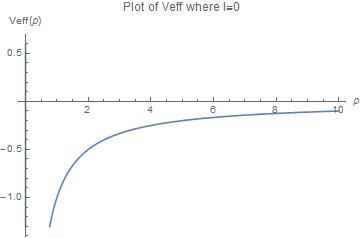
\includegraphics[width=4.5in]{out1}\\
  \caption{$V_{eff}(\rho)$ when $l=0$}\label{out1}
\end{figure}

\begin{figure}
  \centering
  % Requires \usepackage{graphicx}
  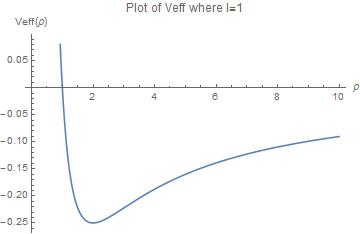
\includegraphics[width=4.5in]{out2}\\
  \caption{$V_{eff}(\rho)$ when $l=1$}\label{out2}
\end{figure}

\begin{figure}
  \centering
  % Requires \usepackage{graphicx}
  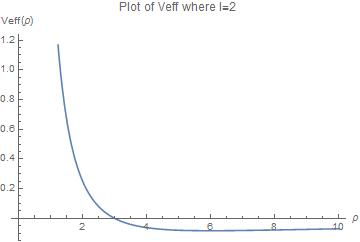
\includegraphics[width=4.5in]{out3}\\
  \caption{$V_{eff}(\rho)$ when $l=2$}\label{out3}
\end{figure}

The plot of $V_{eff}(\rho)$ when $l=0$ is shown in \ref{out1}

The plot of $V_{eff}(\rho)$ when $l=1$ is shown in \ref{out2}

The plot of $V_{eff}(\rho)$ when $l=2$ is shown in \ref{out3}\\

The code for finding and plotting $u(\rho)$ is:

\begin{lstlisting}[language=Mathematica,frame=single]
l := 0
\[Epsilon] := -0.5
ep := $MachineEpsilon
NDSolve[{-u''[\[Rho]]/2+(Veff[\[Rho]]-
\[Epsilon])*u[\[Rho]] == 0,
  u[ep] == 0, u'[ep] == 2}, u, {\[Rho], ep, 10} ]
Plot[u[\[Rho]] /. %, {\[Rho], ep, 10},
 AxesLabel -> {"\[Rho]", "u[\[Rho]]"},
 PlotLabel ->
  "Plot of u[\[Rho]] when l=" <> ToString[l] <>
  " and \[Epsilon]=" <> ToString[\[Epsilon]]]
\end{lstlisting}

Since $u(\rho)$ is singular, ep, which is a number slightly larger than 0, is used here

\subsection*{(c)}
From the property of wave functions, we know that $\lim_{\rho \rightarrow \infty} u(\rho)=0$ must be true

In addition, when n=1, there are no node

When n=2, there is one node

When n=3, there are two nodes

From the differential equation shown in part (b), we know that the eigenvalue is $\epsilon$

When $l=0$, the three eigenvalues occur at n=1,2,3 respectively\\

\begin{figure}
  \centering
  % Requires \usepackage{graphicx}
  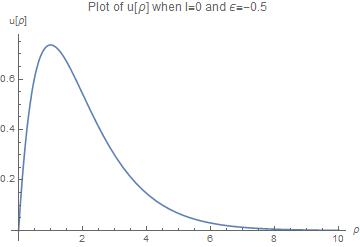
\includegraphics[width=4.5in]{out4}\\
  \caption{$u(\rho)$ when $l=0$ and $n=1$}\label{out4}
\end{figure}

Through experiments, I got the following approximated results:

When $l=0$ and $n=1$, the eigenvalue $\epsilon \approx -0.5$. The graph is shown in Figure \ref{out4}

\begin{figure}
  \centering
  % Requires \usepackage{graphicx}
  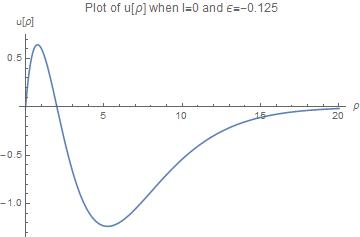
\includegraphics[width=4.5in]{out5}\\
  \caption{$u(\rho)$ when $l=0$ and $n=2$}\label{out5}
\end{figure}

When $l=0$ and $n=2$, the eigenvalue $\epsilon \approx -0.125$. The graph is shown in Figure \ref{out5}

\begin{figure}
  \centering
  % Requires \usepackage{graphicx}
  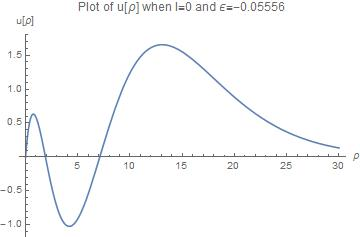
\includegraphics[width=4.5in]{out6}\\
  \caption{$u(\rho)$ when $l=0$ and $n=3$}\label{out6}
\end{figure}

When $l=0$ and $n=3$, the eigenvalue $\epsilon \approx -0.05556$. The graph is shown in Figure \ref{out6}\\

\begin{figure}
  \centering
  % Requires \usepackage{graphicx}
  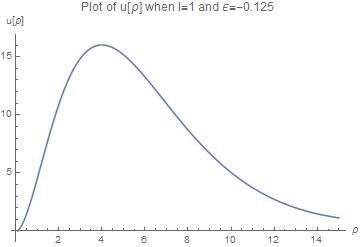
\includegraphics[width=4.5in]{out7}\\
  \caption{$u(\rho)$ when $l=1$ and $n=2$}\label{out7}
\end{figure}

When $l=1$ and $n=2$, the eigenvalue $\epsilon \approx -0.125$. The graph is shown in Figure \ref{out7}

\begin{figure}
  \centering
  % Requires \usepackage{graphicx}
  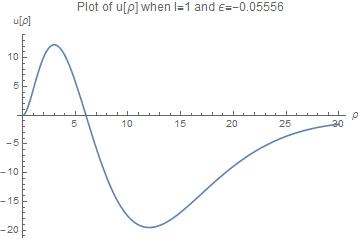
\includegraphics[width=4.5in]{out8}\\
  \caption{$u(\rho)$ when $l=1$ and $n=3$}\label{out8}
\end{figure}

When $l=1$ and $n=3$, the eigenvalue $\epsilon \approx -0.05556$. The graph is shown in Figure \ref{out8}

\begin{figure}
  \centering
  % Requires \usepackage{graphicx}
  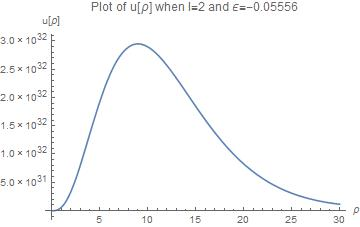
\includegraphics[width=4.5in]{out9}\\
  \caption{$u(\rho)$ when $l=2$ and $n=3$}\label{out9}
\end{figure}

When $l=2$ and $n=3$, the eigenvalue $\epsilon \approx -0.05556$. The graph is shown in Figure \ref{out9}

\subsection*{(d)}

$\because \epsilon=\frac{E}{e^2/4\pi \epsilon_0 a_0}$ and $\frac{e^2}{4\pi \epsilon_0 a_0}=\frac{\hbar^2}{m_e a_0^2}$

$\therefore E=\frac{\hbar \epsilon}{m_e a_0^2}$ where $m_e=9.109*10^{-31} kg$ and $a_0=0.529*10^{-10} m$

When $\epsilon=-0.5$, $E \approx -2.18133*10^{-18}J = -13.61479 eV$

When $\epsilon=-0.125$, $E \approx -5.45333*10^{-19}J = -3.403701 eV$

When $\epsilon=-0.05556$, $E \approx -2.4239*10^{-19}J = -1.512879 eV$

Therefore:

\begin{tabular}{|c|c|c|c|}
  \hline
  % after \\: \hline or \cline{col1-col2} \cline{col3-col4} ...
  Spectroscopic Label & Number of Nodes & $E_{n-calculated} (eV)$ & $E_{n-expected} (eV)$ \\
  \hline
  1s & 0 & $-13.61479$ & $-13.6$ \\
  \hline
  2s & 1 & $-3.403701$ & $-3.4$ \\
  \hline
  2p & 0 & $-3.403701$ & $-3.4$ \\
  \hline
  3s & 2 & $-1.512879$ & $1.511$ \\
  \hline
  3p & 1 & $-1.512879$ & $1.511$ \\
  \hline
  3d & 0 & $-1.512879$ & $1.511$ \\
  \hline
\end{tabular}

From the table given above, we can know the calculated values of energies match the expected values

When $\rho$ approaches 0, $u(\rho)$ approaches to a number larger than 0 when $l=0$. However, $u(\rho)$ approaches 0 when $\rho$ approaches when $l=1$ and $l=2$

However, since the question requires us to set $u[0]=0$ in Mathematica, the graph shown in part (c) when $l=0$ has a huge peak near $\rho=0$. When $l=1$ and $l=2$, the wave function correctly approaches 0 as $\rho$ approaches 0. Therefore the wave functions plotted are considered having a correct dependence on r when r approaches 0.

\section{} %3

\subsection*{(a)}

We know that $[L_z,z]=0$, this means

$\langle \psi_{nlm}|[L_z,z]|\psi_{n'l'm'} \rangle = \langle \psi_{nlm}|(L_zz-zL_z)|\psi_{n'l'm'} \rangle = \hbar m\langle \psi_{nlm}|z|\psi_{n'l'm'} \rangle - \langle \psi_{nlm}|z|\psi_{n'l'm'} \rangle \hbar m' = \hbar(m-m')\langle \psi_{nlm}|z|\psi_{n'l'm'} \rangle = 0$

Therefore this matrix element is zero unless $m=m'$

%We know that $\psi_{nlm}(r,\theta,\phi)= R_{nl}(r)Y_{lm}(\theta,\phi)$
%
%$\therefore \langle \psi_{nlm}|z|\psi_{n'l'm'} \rangle = \int \int \int \psi^{*}_{nlm}z\psi_{n'l'm'} r^2 \sin \theta dr d\theta d\phi=z\delta_{nn'} \delta_{ll'} \delta_{mm'}$
%
%Since the z component is determined by the azimuthal quantum number m and $\delta_{mm'}=1$ only if $m=m'$, this matrix element is zero unless $m=m'$

\subsection*{(b)}

From the equation of radial wave function, we get:

$R_{10}=2 a^{-3/2} \exp \left(-\frac{r}{a}\right)$

$R_{20}= \frac{a^{-3/2} \left(1-\frac{0.5 r}{a}\right) \exp \left(-\frac{r}{2 a}\right)}{\sqrt{2}}$

$R_{21}=\frac{a^{-3/2} r \exp \left(-\frac{r}{2 a}\right)}{\sqrt{24} a}$

$R_{30}=\frac{2 a^{-3/2} \left(\frac{2}{27} \left(\frac{r}{a}\right)^2-\frac{2 r}{3 a}+1\right) \exp \left(-\frac{r}{3 a}\right)}{\sqrt{27}}$

$R_{31}=8/(27*\sqrt{6})*a^{-3/2}*(1 - (1/6)*(r/a))*(r/a)*\exp[-r/(3*a)]$

$R_{32}=4/(81*\sqrt{30})*a^{-3/2}*(r/a)^2*\exp[-r/(3*a)]$

Using mathematica, we get:

\textbf{(i)}

$\langle \psi_{200}|z|\psi_{100} \rangle = \int_{0}^{2\pi} \int_{0}^{\pi} \int_{0}^{\infty} R^{*}_{20}Y^{*}_{00}R_{10}Y_{00} r^2 \sin \theta r \cos \theta dr d\theta d\phi=0$

\textbf{(ii)}

$\langle \psi_{210}|z|\psi_{100} \rangle = \int_{0}^{2\pi} \int_{0}^{\pi} \int_{0}^{\infty} R^{*}_{21}Y^{*}_{10}R_{10}Y_{00} r^2 \sin \theta r \cos \theta dr d\theta d\phi=\frac{128 \sqrt{2} a}{243}$

\textbf{(iii)}

$\langle \psi_{300}|z|\psi_{100} \rangle = \int_{0}^{2\pi} \int_{0}^{\pi} \int_{0}^{\infty} R^{*}_{30}Y^{*}_{00}R_{10}Y_{00} r^2 \sin \theta r \cos \theta dr d\theta d\phi=0$

\textbf{(iv)}

$\langle \psi_{310}|z|\psi_{100} \rangle = \int_{0}^{2\pi} \int_{0}^{\pi} \int_{0}^{\infty} R^{*}_{31}Y^{*}_{10}R_{10}Y_{00} r^2 \sin \theta r \cos \theta dr d\theta d\phi=\frac{27 a}{64 \sqrt{2}}$

\textbf{(v)}

$\langle \psi_{320}|z|\psi_{100} \rangle = \int_{0}^{2\pi} \int_{0}^{\pi} \int_{0}^{\infty} R^{*}_{32}Y^{*}_{20}R_{10}Y_{00} r^2 \sin \theta r \cos \theta dr d\theta d\phi=0$

\textbf{(vi)}

$\langle \psi_{210}|z|\psi_{200} \rangle = \int_{0}^{2\pi} \int_{0}^{\pi} \int_{0}^{\infty} R^{*}_{21}Y^{*}_{10}R_{20}Y_{00} r^2 \sin \theta r \cos \theta dr d\theta d\phi=-3 a$

According to equation 4.32 in textbook, we know that $Y_l^m \cos(\theta)= AY_{l+1}^m+B$ where A,B are constants

$\therefore \langle Y_l^m|z|Y_{l'}^{m'} \rangle = K\delta_{l+1,l'}\delta{m,m'}$ or $K'\delta_{l,l'+1}\delta{m,m'}$ where $K$ and $K'$ are constants

Therefore, as for the matrix elements, $m=m'$ should be true and $|l-l'|=1$ should also be true

\section{} %4

\subsection*{(a)}

We know that $\vec{B}= B\hat{z}$ and $\vec{r}= x\hat{x}+ y\hat{y}+z\hat{z}$

$\therefore \vec{A}=\frac{1}{2} \left( \vec{B} \times \vec{r} \right) = \frac{1}{2} \left| 
\begin{array}{ccc}
\hat{x} & \hat{y} & \hat{z} \\
0 & 0 & B \\
x & y & z
\end{array}
\right|= \frac{1}{2} \left(-By \hat{x}+ Bx\hat{y} \right)= \frac{B}{2}(-y \hat{x}+x\hat{y})$

\subsection*{(b)}

The $\vec{p}$ operator can be written as $\vec{p} = -i\hbar \vec{\bigtriangledown}$

$\vec{A}= (-\frac{1}{2} By + \frac{\partial}{\partial x} (-\frac{1}{2} Bxy) )\hat{x}+ (\frac{1}{2} Bx + \frac{\partial}{\partial y} (-\frac{1}{2} Bxy)) \hat{y} + \frac{\partial}{\partial z} (-\frac{1}{2} Bxy) \hat{z}= -By \hat{x}$

$\Phi=\frac{\partial}{\partial t}=0$

$\therefore H=\frac{1}{2m} \left( \vec{p}^2 + e\vec{A}\cdot \vec{p} + e\vec{p}\cdot\vec{A} + e^2|\vec{A}|^2 \right)= -\frac{\hbar^2}{2m} \vec{\bigtriangledown}^2 + \frac{i\hbar eBy}{2m}\frac{\partial}{\partial x} + \frac{i\hbar e}{2m} \frac{\partial By}{\partial}  + \frac{e^2 B^2 y^2}{2m}= -\frac{\hbar^2}{2m} \vec{\bigtriangledown}^2 + \frac{i\hbar eBy}{2m}\frac{\partial}{\partial x}  +\frac{e^2 B^2 y^2}{2m}$

\subsection*{(c)}

From the Hamiltonian in part (b), we get:

$H\psi(x,y)= -\frac{\hbar^2}{2m} \vec{\bigtriangledown}^2 \psi(x,y) + \frac{i\hbar eBy}{2m}\frac{\partial}{\partial x} \psi(x,y) +\frac{e^2 B^2 y^2}{2m} \psi(x,y) = 
-\frac{\hbar^2}{2m}( \frac{\partial^2}{\partial x^2} e^{ikx} f(y) + e^{ikx} \frac{\partial^2}{\partial y^2}  f(y)) + \frac{i\hbar eBy}{2m}\frac{\partial}{\partial x} e^{ikx} f(y) + \frac{e^2 B^2 y^2}{2m} e^{ikx} f(y) =
 -\frac{\hbar^2}{2m}( -k^2 e^{ikx} f(y) + e^{ikx} f''(y)) - \frac{k\hbar eBy}{2m} e^{ikx} f(y) + \frac{e^2 B^2 y^2}{2m} e^{ikx} f(y) = -\frac{\hbar^2}{2m} \frac{\partial^2}{\partial y^2} \psi + \frac{1}{2} m \frac{e^2 B^2}{m^2} y^2\psi + \frac{\hbar^2 k^2 -k\hbar eBy}{2m} \psi $
 
 The second term is indeed the potential $\frac{1}{2} m \omega_c^2 x^2 \psi$
 
 $\therefore \boxed{\omega_c=\frac{eB}{m}}$

\section{} %5

We know that $\hat{n}= \sin(\theta)\cos(\phi)\hat{x}+ \sin(\theta)\sin(\phi)\hat{y} + \cos(\theta)\hat{z}$

$\therefore s_n = \vec{s}\cdot\hat{n} = s_x\sin(\theta)\cos(\phi) + s_y\sin(\theta)\sin(\phi) + s_z \cos(\theta) = \left(
\begin{array}{cc}
 0 & \frac{\hbar }{2} \\
 \frac{\hbar }{2} & 0 \\
\end{array}
\right)\sin(\theta)\cos(\phi) + \left(
\begin{array}{cc}
 0 & -\frac{1}{2} (i \hbar ) \\
 \frac{i \hbar }{2} & 0 \\
\end{array}
\right)\sin(\theta)\sin(\phi) + \left(
\begin{array}{cc}
 \frac{\hbar }{2} & 0 \\
 0 & -\frac{\hbar }{2} \\
\end{array}
\right) \cos(\theta) = \frac{\hbar}{2} \left(
\begin{array}{cc}
\cos(\theta) & e^{-i\phi} \sin(\theta) \\
e^{i\phi} \sin(\theta) & \cos(\theta)
\end{array}
\right)$

Let $\lambda$ denote eigenvalue and $c$ denote the eigenvector

Then $\frac{\hbar}{2}\left|
\begin{array}{cc}
\cos(\theta)-\lambda I & e^{-i\phi} \sin(\theta) \\
e^{i\phi} \sin(\theta) & \cos(\theta)-\lambda I
\end{array}
\right|=0$

$\frac{\hbar^2}{4}(\cos(\theta)-\lambda I)(\cos(\theta)-\lambda I)-\frac{\hbar^2}{4}(e^{-i\phi} \sin(\theta))(e^{i\phi} \sin(\theta))=0$

The $s_n$ matrix is input to Mathematica. Using Eigensystem function in Mathematica, we therefore get

$\lambda_1=-\frac{\hbar }{2}$ and $\lambda_2=\frac{\hbar }{2}$

$\because \frac{\hbar}{2} \left(
\begin{array}{cc}
\cos(\theta) & e^{-i\phi} \sin(\theta) \\
e^{i\phi} \sin(\theta) & \cos(\theta)
\end{array}
\right)c_1 = -\frac{\hbar }{2}c_1$ and 
$\frac{\hbar}{2} \left(
\begin{array}{cc}
\cos(\theta) & e^{-i\phi} \sin(\theta) \\
e^{i\phi} \sin(\theta) & \cos(\theta)
\end{array}
\right)c_2 = \frac{\hbar }{2}c_2$

$\therefore c_1=
\left(
\begin{array}{c}
 -\frac{\sin (\theta ) \cos (\phi )-i \sin (\theta ) \sin (\phi )}{\cos (\theta
   )+1} \\
 1 \\
\end{array}
\right)
=\left(
\begin{array}{c}
e^{-i\phi}\sin(\frac{\theta}{2}) \\
-\cos(\frac{\theta}{2}) 
\end{array}
\right)$
 
$c_2=
\left(
\begin{array}{c}
 -\frac{\sin (\theta ) \cos (\phi )-i \sin (\theta ) \sin (\phi )}{\cos (\theta
   )-1} \\
 1 \\
\end{array}
\right)
=\left(
\begin{array}{c}
 \cos(\frac{\theta}{2})\\
 e^{i\phi}\sin(\frac{\theta}{2})
\end{array}
\right)$

Therefore the eigenvalues are $-\frac{\hbar }{2}$ and $\frac{\hbar }{2}$, the corresponding eigenvectors are  
$\left(
\begin{array}{c}
e^{-i\phi}\sin(\frac{\theta}{2}) \\
-\cos(\frac{\theta}{2})
\end{array}
\right)$ and 
$\left(
\begin{array}{c}
 \cos(\frac{\theta}{2})\\
 e^{i\phi}\sin(\frac{\theta}{2})
\end{array}
\right)$

\end{spacing}
\end{document} 